
\textbf{Ejercicio 16.} Hallar el volumen de la región limitada por la esfera
\[
x^2+y^2+z^2=32
\]
y contenida dentro del cono
\[
z=\sqrt{x^2+y^2}.
\]

La superficie $x^2+y^2+z^2=32$ es una esfera de radio $R=4\sqrt{2}$ y el cono $z=\sqrt{x^2+y^2}$ abre hacia los $z$ positivos. La región pedida es la parte de la esfera por encima del cono.

\begin{figure}[htbp]
\centering
\tikzsetnextfilename{ejercicio16_figura}
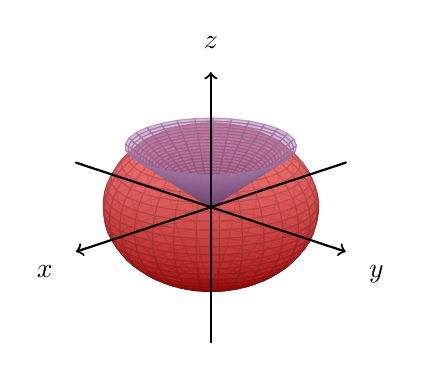
\begin{tikzpicture}[line cap=round, line join=round]
\begin{axis}[
    axis on top,
    view={135}{25}, % Rotamos la cámara: x a la izquierda, y a la derecha
    axis lines=center,
    xmin=-10, xmax=10, % Agrandamos los ejes para que entre el radio de 5.65
    ymin=-10, ymax=10,
    zmin=-10, zmax=10,
    ticks=none,
    xlabel={$x$},
    ylabel={$y$},
    zlabel={$z$},
    axis line style={thick, ->, black},
    every axis x label/.style={at={(ticklabel* cs:1.05)},anchor=north east},
    every axis y label/.style={at={(ticklabel* cs:1.05)},anchor=north west},
    every axis z label/.style={at={(ticklabel* cs:1.05)},anchor=south},
]

% Esfera roja (radio 4*sqrt(2))
\addplot3[
    surf,
    opacity=0.8,
    colormap={redmap}{color=(red!60!black) color=(red!50!white)},
    samples=30,
    domain=0:360,
    y domain=0:180,
    z buffer=sort
]
({4*sqrt(2)*cos(x)*sin(y)}, {4*sqrt(2)*sin(x)*sin(y)}, {4*sqrt(2)*cos(y)});

% Cono violeta (z = sqrt(x^2 + y^2))
% Lo graficamos hasta z=4.5 para que pase justo la intersección
\addplot3[
    surf,
    opacity=0.6,
    colormap={purplemap}{color=(violet!50!black) color=(violet!40!white)},
    samples=30,
    domain=0:360,
    y domain=0:4.5,
    z buffer=sort
]
({y*cos(x)}, {y*sin(x)}, {y});

\end{axis}
\end{tikzpicture}
\caption{Representación de la región pedida. \href{https://www.geogebra.org/m/pvzc3wke}{Ver en GeoGebra}}
\end{figure}


La intersección entre  ambas superficies se obtiene de
\[
r=z, \quad r^2+z^2=32 \Rightarrow 2r^2=32 \Rightarrow r=4.
\]

\textbf{En coordenadas cartesianas:}
\[
x^2+y^2+z^2 \le 32, \quad z \ge \sqrt{x^2+y^2}.
\]

\[
D=\left\{(x,y,z):
0\le x\le 4,\;
-\sqrt{16-x^2}\le y\le \sqrt{16-x^2},\;
\sqrt{x^2+y^2}\le z\le \sqrt{32-x^2-y^2}
\right\}
\]

\[
V=\int_{-4}^{4}
\int_{-\sqrt{16-x^2}}^{\sqrt{16-x^2}}
\int_{\sqrt{x^2+y^2}}^{\sqrt{32-x^2-y^2}}
dz\,dy\,dx.
\]

\bigskip

\textbf{En coordenadas cilíndricas:}
\[
x = r\cos\theta, \quad y = r\sin\theta, \quad z = z
\]

\[
r^2+z^2=32, \quad z=r,
\]

\[
0\le\theta\le2\pi,\quad 0\le r\le4,\quad r\le z\le\sqrt{32-r^2},
\]

\[
V=\int_0^{2\pi}\int_0^4\int_r^{\sqrt{32-r^2}} r\,dz\,dr\,d\theta.
\]

\bigskip

\textbf{En coordenadas esféricas:}
\[
x=\rho\sin\varphi\cos\theta,\quad
y=\rho\sin\varphi\sin\theta,\quad
z=\rho\cos\varphi
\]

\[
\rho\cos\varphi=\rho\sin\varphi \Rightarrow \tan\varphi=1 \Rightarrow \varphi=\frac{\pi}{4},
\]

\[
0\le\theta\le2\pi,\quad 0\le\varphi\le\frac{\pi}{4},\quad 0\le\rho\le4\sqrt{2},
\]

\[
V=\int_0^{2\pi}\int_0^{\pi/4}\int_0^{4\sqrt{2}}\rho^2\sin\varphi\,d\rho\,d\varphi\,d\theta.
\]

\bigskip

Calculando:
\[
\int_0^{4\sqrt{2}}\rho^2 d\rho=\frac{128\sqrt{2}}{3}, \quad
\int_0^{\pi/4}\sin\varphi\,d\varphi=1-\frac{\sqrt{2}}{2}, \quad
\int_0^{2\pi}d\theta=2\pi.
\]

\[
V=2\pi\cdot\frac{128\sqrt{2}}{3}\left(1-\frac{\sqrt{2}}{2}\right)
=\frac{256\pi}{3}(\sqrt{2}-1).
\]

\[
\boxed{V=\frac{256\pi}{3}(\sqrt{2}-1)}
\]
